\scanpage{173}

\margin{\figure{\begin{tikzpicture}[baseline=0pt]\draw (0,0) circle (0.04);\draw (0.04,0)--(0.8,0);\end{tikzpicture}} $\omega_l(q)=$ ordre de $q$ mod $l$ dans $(\mathbf Z/l\mathbf Z)^*$.}

\diagram{\begin{tikzcd}[column sep=large]
k=\mathbf F_q \arrow[r,no head] & \bar k
\end{tikzcd}}
\[
\pi\simeq\widehat{\mathbf Z}
\]
engendré par $f=\operatorname{frob}^q$

$M$ un $\mathbf Z_l$-module de t.f. sur lequel $\pi$ opère continûment.

\[
H^0(\pi,M)=M^\pi=M^{(1-f)}=\operatorname{Ker}(1-f)_M
\]
\[
H^1(\pi,M)=M'_\pi=M_{(1-f)}=\operatorname{Coker}(1-f)_M=M/(1-f)M
\]
\[
H^i(\pi,M)=0\quad\text{si }i\geq2
\]

\[
H^0(\pi,\mathbf Z_l(n))=0\quad\text{si }n\neq0,\qquad=\mathbf Z_l\quad\text{si }n=0
\]
\[
H^1(\pi,\mathbf Z_l(n))\underset{\text{non canoniquement}}{=}
\mathbf Z_l/(1-q^n)\mathbf Z_l
=\begin{cases}
\mathbf Z_l&\text{si }n=0\\
0&\text{si }l\nmid(1-q^n)\quad\text{i.e. }\underset{\deleted{\unsure{?}}}{n\not\equiv0}\ (\omega_l(q))\\
\mathbf Z/l^{v_l(1-q^n)}&\text{si }\underbrace{l\mid1-q^n}_{\text{i.e. }n\equiv0\ (\omega_l(q))},\ n\neq0
\end{cases}
\]
\margin{\figure{\begin{tikzpicture}[baseline=0pt]\draw (0,0) circle (0.04);\draw (0.04,0)--(0.8,0);\end{tikzpicture}}}

\[
\left\{\begin{aligned}
&H^i(\pi,\mathbf Q_l(n))=0\quad\text{si }n\neq0,\quad\text{quel que soit }i\\
&H^0(\pi,\mathbf Q_l)=\mathbf Q_l\unsure{4|!},\quad H^1(\pi,\mathbf Q_l)=\mathbf Q_l
\end{aligned}\right.
\]

\deleted{$H^i(\pi,\uline{\mathbf Z}(n)$}
\[
\left\{\begin{aligned}
&\mathbb H^i(\mathbf F_q,\underset{\sim}{\mathbf Q}(n))=0\quad\text{si }n\neq0,\quad\text{quel que soit }i\\
&\mathbb H^0(\mathbf F_q,\underset{\sim}{\mathbf Q})=\mathbf Q,\quad\mathbb H^1(\mathbf F_q,\underset{\sim}{\mathbf Q})=\underset{\sim}{\mathbf Q}.
\end{aligned}\right.
\]
\[
\left\{\begin{aligned}
&\mathbb H^0(\mathbf F_q,\underset{\sim}{\deleted{\mathbf Q}\inserted{\mathbf Z}})=\mathbf Z\ (\text{mod }\unsure{p\text{-grps}|p\text{-groupes}}?),\quad
\mathbb H^1(\mathbf F_q,\underset{\sim}{\mathbf Z})=\mathbf Z\ (\text{mod }\unsure{p\text{-grps}|p\text{-groupes}}?)\\
&H^0(\mathbf F_q,\underset{\substack{\vert\\\inserted{n\neq0}}}{\underset{\sim}{\mathbf Z}(n)})=0\ (\text{id}),\quad
\mathbb H^1(\mathbf F_q,\underset{\substack{\vert\\\inserted{n\neq0}}}{\underset{\sim}{\mathbf Z}(n)})=\mathbf Z/(1-q^n)\mathbf Z\ (\text{mod }\unsure{p\text{-grps}|p\text{-groupes}}?)
\end{aligned}\right.
\]

\figure{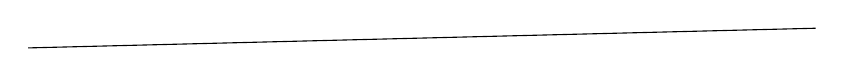
\begin{tikzpicture}\draw (0,0)--(10,0.25);\end{tikzpicture}}

\[
\mathbb H^i(\operatorname{Spec}\mathbf Z,\mathbf Z(1))=\begin{cases}0&\underset{\text{
\begin{tikzpicture}[baseline=0pt]\draw[line width=0.7pt] (0,0)--(0.28,0.08)--(0.04,-0.05)--(0.32,-0.14)--(0.28,0.03)--(0.12,-0.09)--(0.35,-0.18)--(0.26,0.02);\end{tikzpicture}}}{\text{si }}i\neq3\\\mathbf Z&\text{si }i=3\end{cases}
\]
\[
\mathbb H^i(\operatorname{Spec}\mathbf Z,\mathbf Z)=\begin{cases}0&\text{si }i\neq0\\\mathbf Z&\text{si }i=0\end{cases}
\]
\margin{$H^i(\operatorname{Spec}(\mathbf Z),\mathbf Q(n))\xrightarrow{\sim}H^i(U,\mathbf Q(n))$ si $U$ ouvert de Zariski de $\operatorname{Spec}\mathbf Z$ et $n\neq0$ (tout $i$).}

\margin{172}
